\section{Klasser}
En HiFi-forstærkers udgangstrin kan designes på forskellige måder alt efter hvilke karakteristika man ønsker at opnå. De forskellige designs er opdelt i klasser. I dette afsnit vil der blive taget udgangspunkt i grundkoblinger, som viser funktionaliteten af de forskellige klasser. 
I dette afsnit vil der blive gjort rede for de gængse klassifikationer, som har med analogt opbyggede forstærkere at gøre, og forklare hvilke fordele og ulemper der er med dem. Der vil, på baggrund af dette afsnit, blive valgt en endelig udgangstrinsklasse til dette projekts HiFi-forstærker hvilket vil blive opstillet, som et krav i kravspecifikationen.

\subsection{Klasse A}

En klasse A forstærker er opbygget af to NPN transistorer, Q1 og Q2, i en emitterfølgerkobling, som vist på figur \ref{fig:classa}. En konstant strøm løber gennem Q2, da $v_{BE2}$ er konstant. Inputsignalet kommer ind på Q1's base og styrer således strømmen der kan løbe gennem Q1 og loadmodstanden. 
Klasse A udgangstrin er et godt valg rent forvrængningsmæssigt, hele inputsignalet bliver gengivet på output, men er dog ikke et det mest benyttede i HiFi-forstærkere. Årsagen til dette er at Q2 konstant leder en strøm, som er uafhængig af inputsignalets styrke eller om der overhovedet er et inputsignal til stede. Derfor er virkningsgraden af et klasse A udgangstrin ikke særlig høj, sammenlignet med nogle af de andre typer. Den maksimale teoretiske virkningsgrad af et klasse A udgangstrin er giver ved ligning \ref{eq:classa}.

\begin{eqnarray}
\eta=\frac{1}{4} \cdot \frac{\widehat{V}_o^2}{I \cdot R_L \cdot V_{CC}}  \label{eq:classa}
\end{eqnarray}


Da den mindst afsatte effekt opnås når Q1 er helt lukket, altså: $ \widehat{V}_o=V_{CC}=I \cdot R_L $, bliver den maksimale virkningsgrad 25\%.

\begin{figure}[h]
\centering
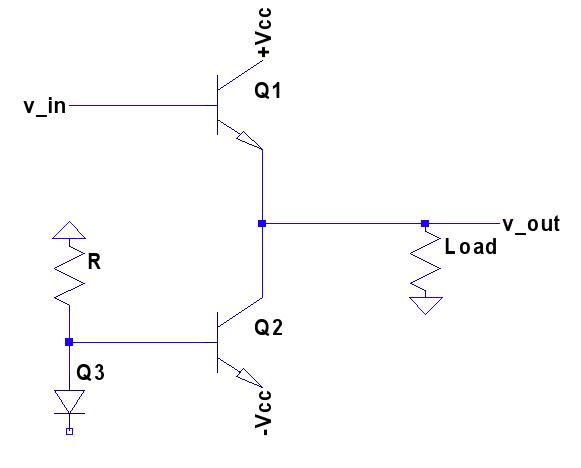
\includegraphics[scale=.35]{indledende_analyse/klasser/classa.png}
\caption{Klasse A forstærker kredsløb.}
\label{fig:classa}
\end{figure}


\subsection{Klasse B}
En klasse B forstærker er opbygget af to transistorer, en NPN (Q1) og en PNP (Q2), som vist på figur \ref{fig:classb}. Når input spændingen overstiger ca. 0,5 V vil Q1 begynde at lede strøm til loadmodstanden mens Q2 er lukket. Kommer input spændingen under -0,5 V vil Q2 lede, men da Q2 er en PNP vil den trække strøm mod -Vcc hvormed der trækkes strøm fra loadmodstanden. Når Q2 leder er Q1 lukket. 
Et klasse B udgangstrin er mere forvrængende end et klasse A fordi den har et dødt område på  $\pm$ saturationspændingen, hvilket vil sige at der først vil optræde et output når inputtet overstiger dette dødområde.  Der afsættes dog ikke nær så meget effekt i en klasse B forstærker når inputspændingen er 0 V, som i en klasse A. Dette skyldes at ingen af transistorerne leder strøm når $v_{BE} $ er under saturationspændingen. Virkningsgraden for et klasse B udgangstrin er givet ved ligning \ref{eq:classb}.

\begin{eqnarray}
\eta=\frac{1}{4} \cdot \frac{\widehat{V}_o^2}{I \cdot R_L \cdot V_{CC}}  \label{eq:classa}
\end{eqnarray}

\begin{figure}[h]
\centering
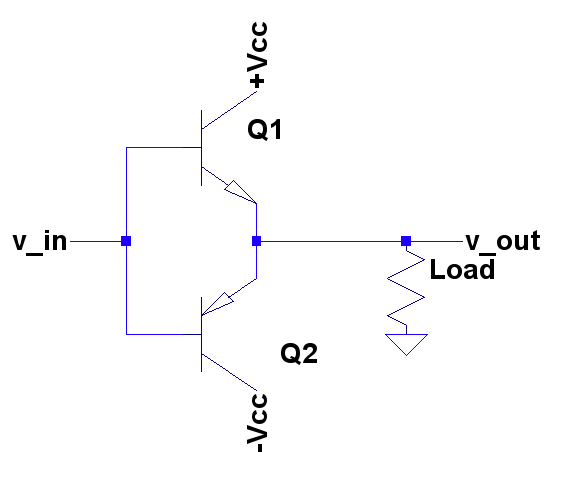
\includegraphics[scale=.35]{indledende_analyse/klasser/classb.png}
\caption{Klasse B forstærker kredsløb.}
\label{fig:classb}
\end{figure}

\subsection{Klasse AB}

Et klasse AB udgangstrin er næsten opbygget på samme måde som et klasse B, med den forskel at potentialet på Q1 og Q2's base er hævet til saturationspændingen når inputspændingen er 0 V. Ved at gøre dette elimineres dødområdet, som klasse B udgangstrinnet har, hvorved forvrængningen formindskes. 
Klasse AB er det oftest benyttede i moderne HiFi-forstærkere grundet den lave forvrængning kontra energiforbrug. \fixme{ref til sedra/smith}

\begin{figure}[h]
\centering
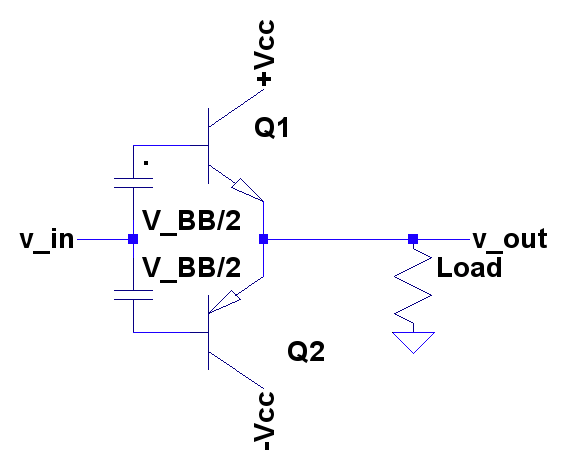
\includegraphics[scale=.35]{indledende_analyse/klasser/classab.png}
\caption{Klasse AB forstærker kredsløb.}
\label{fig:classab}
\end{figure}

\fixme{skriv om virkningsgrad i stedet for at snakke løst om effektforbrug}
\fixme{indsæt grafer som viser outputtet af de forskellige}
